\chapter{Iterazione 1}

\section{Introduzione}
Nella prima iterazione sono stati scelti i seguenti casi d'uso:

\begin{itemize}
    \item Gestione barche [Proprietario]
    \item Calendario delle uscite [Proprietario]
    \item Registrazione [Utente]
\end{itemize}
Dopo averli descritti in maniera testuale, prima di implementarli si è passati alla realizzazione del diagramma dei componenti e del deployment diagram.

\section{UC1: Gestione barche}
Il proprietario del diving center deve avere una visione completa e generale delle sue barche.
Accedendo all'applicazione deve poter visualizzare tutte le barche presenti e per ognuna queste caratteristiche:

\begin{itemize}
    \item Nome della barca
    \item Modello della barca
    \item Numero posti disponibili sulla barca
    \item Altre caratteristiche TODO
\end{itemize}

Oltre alla visualizzazione, il proprietario deve poter modificare le imbarcazioni già presenti nel sistema.
Tali modifiche possono essere dovute a cambiamenti strutturali della barca, per esempio la riduzione del numero di posti disponibili
o all'eliminazione di una barca dal sistema.
Quest'ultima può essere definitiva o temporanea. L'eliminazione è definitiva se la barca non è più agibile o perché viene sostituita da un'altra;
è temporanea nel caso in cui sia necessaria attività di manutenzione.

\section{UC2: Calendario delle uscite}
L'applicazione deve poter semplificare la gestione e l'organizzazione delle uscite al proprietario del diving center.
\\Da questo punto di vista l'applicazione deve fungere da calendario, mettendo a disposizione le seguenti funzionalità:

\begin{itemize}
    \item L'inserimento di una data in cui si rende disponibile la prenotazione di uscite, indicando i turni con i relativi orari e durate.
    \item Visualizzazione di tutte le date e turni messi a disposizione.
    \item La modifica o la cancellazione delle date e dei turni, in seguito a cambiamenti climatici o altri imprevisti.
\end{itemize}

\section{UC3: Registrazione dell'utente}
Linda

\section{UML Component diagram}
I casi d'uso scelti in questa prima iterazione vengono rappresentati sottoforma di componenti nel diagramma in Figura~\ref{fig:componentDiagram}.
Si è scelto di suddividire i caso d'uso in componenti:

\begin{itemize}
    \item <<boundary>> rappresentati dai componenti lato front-end con cui gli attori si interfacciano direttamente. Tali componenti richiedono delle interfacce al back-end.
    \item <<control>> rappresentati dai componenti lato back-end che forniscono delle API al front-end, richiedonone a loro volta al database.
    \item <<data>> rappresentato dal database in cui verranno memorizzati i dati delle barche, il calendario delle uscite e i dati dell'utente in occasione della registrazione.
\end{itemize}

\begin{figure}[h]
    \centering
    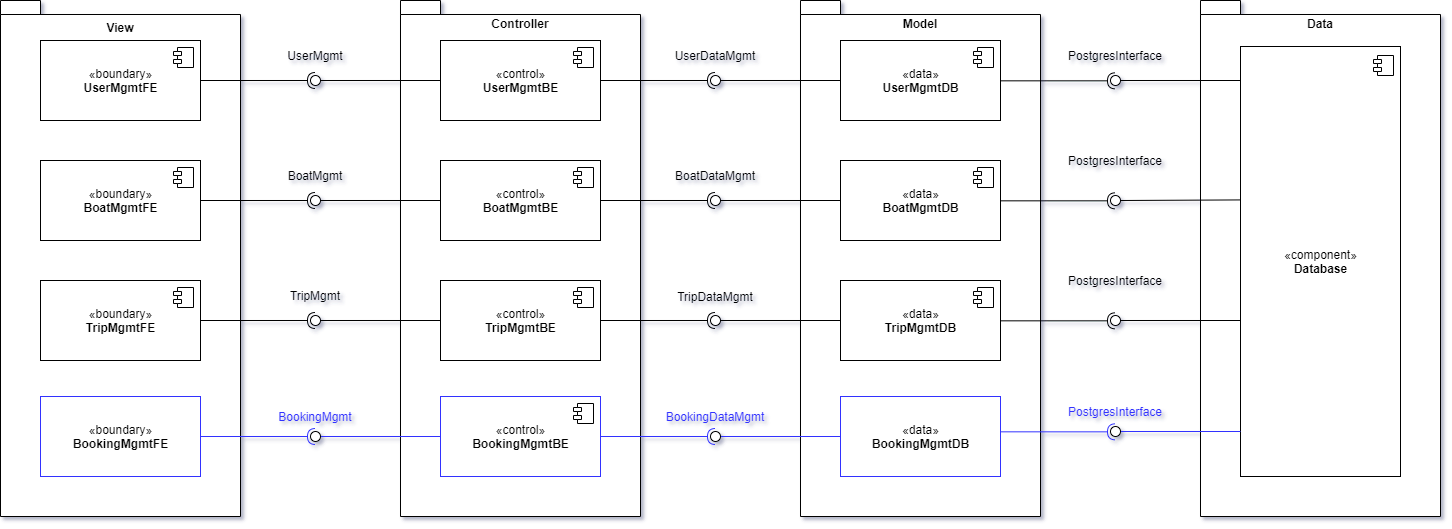
\includegraphics[scale=0.27]{ComponentDiagram_v1.png}
    \caption{Diagramma dei componenti UML.}\label{fig:componentDiagram}
\end{figure}

\section{UML Deployment diagram}
I componenti descritti precedentemente vengono istanziati nel Deployment diagram. In Figura~\ref{fig:deploymentDiagram} vengono mostrati i componenti contenuti nei seguenti nodi:

\begin{itemize}
    \item Cellulare proprietario è il nodo su cui l'admin del sistema potrà gestire le barche e il calendario delle uscite.
    \item Cellulare utente è il nodo su cui una persona potrà registrarsi alla piattaforma.
    \item Web server fornisce le API richieste dall'applicativo lato front-end.
    \item Database funge da storage dei dati.
\end{itemize}

\begin{figure}[h]
    \centering
    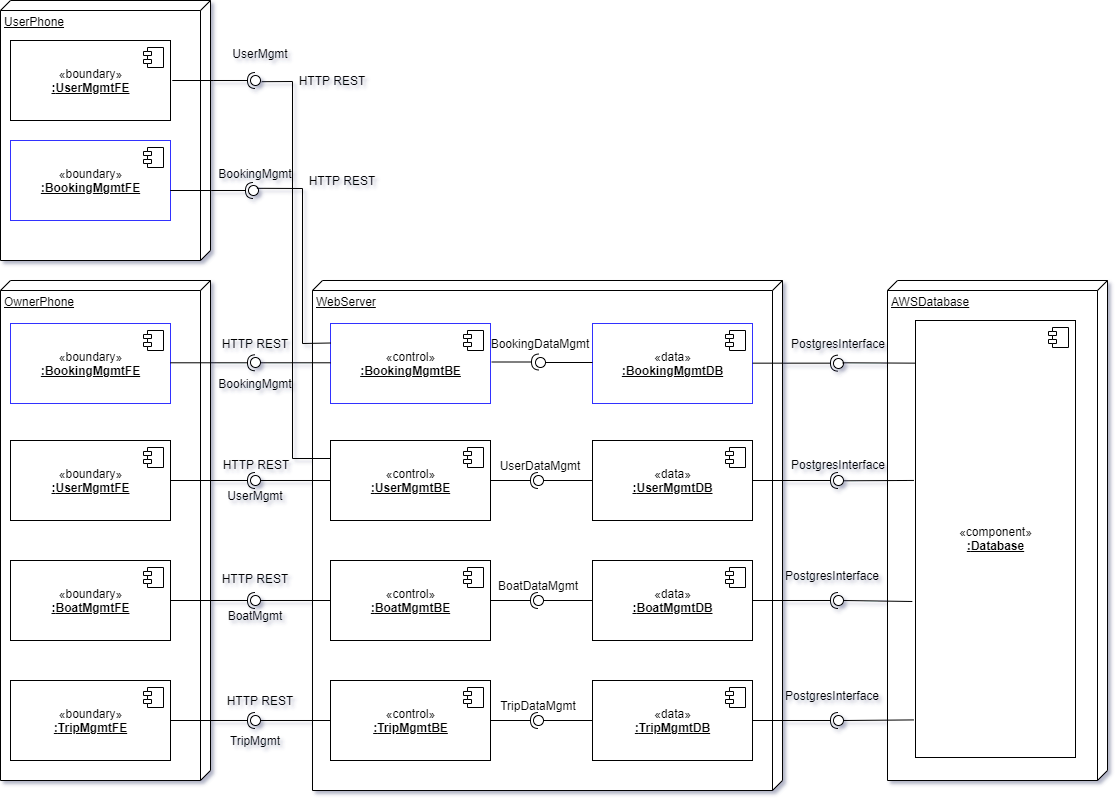
\includegraphics[scale=0.4]{DeploymentDiagram_v1.png}
    \caption{Deployment diagram UML.}\label{fig:deploymentDiagram}
\end{figure}